% This must be in the first 5 lines to tell arXiv to use pdfLaTeX, which is strongly recommended.
\pdfoutput=1
% In particular, the hyperref package requires pdfLaTeX in order to break URLs across lines.

\documentclass[11pt]{article}

% Remove the "review" option to generate the final version.
\usepackage[review]{acl}

% Standard package includes
\usepackage{times}
\usepackage{latexsym}

% For proper rendering and hyphenation of words containing Latin characters (including in bib files)
\usepackage[T1]{fontenc}
% For Vietnamese characters
% \usepackage[T5]{fontenc}
% See https://www.latex-project.org/help/documentation/encguide.pdf for other character sets

% This assumes your files are encoded as UTF8
\usepackage[utf8]{inputenc}

% This is not strictly necessary, and may be commented out,
% but it will improve the layout of the manuscript,
% and will typically save some space.
\usepackage{microtype}

\usepackage{graphicx}

% If the title and author information does not fit in the area allocated, uncomment the following
%
%\setlength\titlebox{<dim>}
%
% and set <dim> to something 5cm or larger.
\title{Syntax-Based Concept Alignment for Domain-Specific Machine Translation}

% Author information can be set in various styles:
% For several authors from the same institution:
% \author{Author 1 \and ... \and Author n \\
%         Address line \\ ... \\ Address line}
% if the names do not fit well on one line use
%         Author 1 \\ {\bf Author 2} \\ ... \\ {\bf Author n} \\
% For authors from different institutions:
% \author{Author 1 \\ Address line \\  ... \\ Address line
%         \And  ... \And
%         Author n \\ Address line \\ ... \\ Address line}
% To start a seperate ``row'' of authors use \AND, as in
% \author{Author 1 \\ Address line \\  ... \\ Address line
%         \AND
%         Author 2 \\ Address line \\ ... \\ Address line \And
%         Author 3 \\ Address line \\ ... \\ Address line}
% TODO: authors info
\author{First Author \\
  Affiliation / Address line 1 \\
  Affiliation / Address line 2 \\
  Affiliation / Address line 3 \\
  \texttt{email@domain} \\\And
  Second Author \\
  Affiliation / Address line 1 \\
  Affiliation / Address line 2 \\
  Affiliation / Address line 3 \\
  \texttt{email@domain} \\}

\begin{document}
\maketitle
\begin{abstract}
In grammar-based domain-specific machine translation, constructing high-quality translation lexica is a crucial but time consuming task requiring significant linguistic knowledge. 
In presence of a corpus of parallel example sentences, statistical word and phrase alignment tools allow to automate part of this process, but are not suitable for small datasets and often fail to identify discontinuous multiword correspondences. 
Addressing both problems, we propose a data-driven, syntax-based approach to the automation of this task and put it to the test in a simple grammar-based translation pipeline.
\end{abstract}

\section{Introduction}
Grammar-based translation pipelines such as those based on Grammatical Framework (GF) \cite{TODO:} have been successfully employed in domain-specific Machine Translation (MT). 
What makes these systems well suited to the task is the fact that, when we constrain ourselves to a specific domain, where precision is most often more important than coverage, they can provide strong guarantees in terms of grammatical correctness. 

Nevertheless, lexical exactness is, in this context, just as important as grammaticality. 
An important part of the design of the Controlled Natural Language (CNL) the grammar in such a system describes becomes, then, the creation of a translation lexicon. 
In many cases, this is done for the most part manually, resulting in a time consuming task requiring significant linguistic knowledge. 
When the grammar is designed based on a parallel corpus of example sentences, it is possible to automate part of this process by means of statistical word and phrase alignment techniques \cite{TODO: a lot}. 
None of them is, however, suitable for the common case in which only a limited number of example sentences is available.

In this paper, we propose an alternative approach to the automation of this task. 
While still being data-driven, our method is grammar-based and, as such, capable of extracting meaningful correspondences even from individual sentence pairs. 

A further advantage of performing syntactic analysis is that we do not have to choose \textit{a priori} whether to focus on the word or phrase level. 
Instead, we can simultaneously operate at different levels of abstraction, thus extracting both single- and multiword, even non-contiguous, correspondences. 

For this reason, we refer to the task our system attempts to automate as \textit{Concept Alignment} (CA). 

This paper is structured as follows. 
Section \ref{methodology} starts by giving an overview of our approach to CA, comparing it to related work, to then focus on our algorithm for extracting correspondences.
It is concluded with a description of our method for converting the alignments obtained in this way to a GF translation lexicon.
After that, Section \ref{evaluation} presents the results of our first evaluation of the system.
Finally, Section \ref{conclusions} consists of a discussion of such results and some ideas for future work. 

\section{Methodology} \label{methodology}
The objective of CA is to find semantical correspondences between parts of multilingual parallel texts. 
We call \textit{concepts} the abstract units of translation, composed of any number of words, identified through this process, and represent them as \textit{alignments}, i.e. tuples of equivalent concrete expressions in different languages.

The basic use case for CA, which we refer to specifically as \textit{Concept Extraction} (CE), is the generation of a translation lexicon from a parallel text. This can be directly compared to the numerous existing word and phrase alignment techniques. 

% potentially move to future work directly
An interesting and less studied variant of CA is \textit{Concept Propagation} (CP), useful for cases where a set of concepts is already known and the goal is to identify the expressions corresponding to each of them in a new language, potentially even working with a different text in the same domain.
While our system implements basic CP functionalities, however, in this paper we focus on CE and restrict its application to bilingual corpora. 

As stated in the Introduction, most existing extraction solutions are based on statistical approaches and are, as a consequence, unsuitable for small datasets. 
Grammar-based approaches, making use of parallel treebanks and collectively referred to as \textit{tree-to-tree alignment methods}, have also been proposed \cite{TODO:}, but have historically suffered from the inconsistencies between the various constituency grammar formalisms used to define grammars for the different languages and from the insufficient degree of robustness of existing parses.

This work is a new attempt in the same direction, enabled by two multilinguality-oriented grammar formalisms developed over the course of the last 25 years: Universal Dependencies (UD) \cite{TODO:} and Grammatical Framework (GF) \cite{TODO:}.

While both formalisms, the former a dependency and the latter a constituency grammar, independently solve the former issue, UD is especially appealing since dependency trees are an easier target for parsing. 
As a consequence, several robust dependency parsers, such as \cite{TODO: UDPipe} and \cite{TODO: Standford} are available.

UD parsing alone would then be sufficient to extract (or propagate) tree-to-tree alignments, but not to automate the generation of a ready-to-use, morphologically-aware translation lexicon. This is where GF comes into play: after correspondences are inferred from a parallel text, our proposed system is able to convert them to GF grammar rules, easy to embed in a domain-specific grammar but also making it possible to immediately evaluate the system by carrying out small-scale translation experiment using pre-existing grammatical constructions implemented in GF's Resource Grammar Library (RGL) \cite{TODO:}. 
This is made possible by \texttt{gf-ud}, a conversion tool described in \cite{TODO:} and \cite{TODO:}.

Concretely, the system we propose requires the following elements, whose reciprocal relations are shown in Figure \ref{overview}: \smallskip

\begin{itemize}
  \item a UD parser
  \item an alignment module based on dependency tree comparison
  \item a program, based on \texttt{gf-ud}, that converts the alignments into GF grammar rules and uses them to construct a translation lexicon
\end{itemize} \smallskip

% TODO: replace CE with CA and omit CP entirely?
\begin{figure}[h]
  \centering
  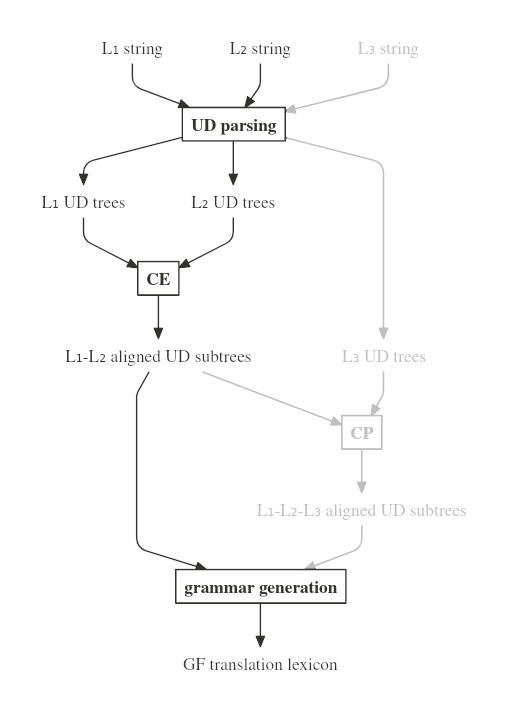
\includegraphics[width=0.45\textwidth]{figures/overview.png}
  \caption[System overview]{System overview. Parts in grey are currently at the prototype stage and will not be further discussed in this paper.} \label{elems}
  \label{overview}
\end{figure}

\subsection{Extracting concepts} 
The core part of the system outlined above is of course the alignment module. In this section, we present our method for extracting alignments from parallel bilingual UD treebanks, which can be obtained from sentence-aligned texts with any UD parser.

The basic extraction algorithm, whose pseudocode is shown in Figure \ref{TODO}, takes as input a list of priority-sorted \textit{alignment criteria}, rules to determine whether two dependency trees should be aligned with each other which we will discuss in greater detail in Section \ref{criteria}, and a pair of UD trees corresponding to the sentences to align.
From an implementation point of view, UD trees are, as in \texttt{gf-ud}, rose trees where each node represents a token,  obtained from the CoNLL-U files produced by the UD parser.

% TODO: add figure comparing tree representations

As a first step, the program checks whether the two full sentence trees can be aligned with each other, i.e. if they match any of the alignment criteria. If this is the case, they are added to a collection of alignments, also represented as a pair of UD trees associated with some metadata, which is what the function will return after aligning all the dependency subtrees. % TODO: explain or omit metadata!

Depending on which alignment criteria they match, the head of the two trees may or may not also be added to such collection. This is important... % TODO:

The same procedure is applied recursively to all pairs of immediate subtrees of each sentence, until the leaves are reached or alignment is no longer possible due to lack of matching criteria.  % TODO: explain & motivate sorting -> maybe say more about UD before?

% TODO: pseudocode

When working on corpora consisting of multiple sentences, this algorithm can be applied in an iterative fashion, so that knowledge gathered when a sentence pair is aligned can be reused when working on the following ones and to keep track of the number of occurrences of each alignment throughout the entire text.

\subsubsection{Alignment criteria} \label{criteria}
While alignment criteria are customizable, to better understand the extraction algorithm described in the above we dedicate this section to describing the ones that are currently used by default.

\paragraph{Matching UD labels}
The most obvious, but also most effective idea is to determine alignability based on comparing the dependency labels of the candidate UD tree pair. 
In particular, according to this idea, two subtrees, in \textit{matching context}, i.e. attached to aligned heads constitute an alignment if their roots share the same dependency label. 
Intuitively, this means that they are in the same relation with their heads.

Note that, since the root of US trees is always attached to a a fake node with an arc labelled \texttt{root}, this criterion also makes it so that full sentences are always considered to align with each other, something which is desirable since we assume the parallel texts that are fed to our program to be sentence-aligned.

\paragraph{Part-Of-Speech equivalence}
CoNNL-U files provide information not only on the syntactic role of the tokens a sentence is composed of, but also on their grammatical categories, represented as Universal Part-Of-Speech (POS) tags. 
Intuitively, if the nodes of two trees in matching contexts have the same POS tags, the two trees are more likely to correspond to each other than if not. 

This is especially true if focus, for instance, solely on the open class words (in the current implementation, defined as in the UD documentation \cite{TODO:}), thus ignoring prepositions, determiners, auxiliary verbs and all other function words, which tend to behave differently across different languages.

As a consequence, a useful relation to define between dependency trees is that of \textit{POS-equivalence}: two dependency trees $t$, $u$ are POS-equivalent if $M_1 = M_2 \neq \emptyset$, where $M_i$ is defined as the multiset of POS tags of all the open class word nodes of $t_i$. 

Applied alone, this criterion can be used to capture correspondences that would be missed by only matching UD labels, thus increasing recall, but a decrease in precision is also to be expected. 
However, since alignment criteria are defined as boolean functions, it is easy to combine them so to apply them simultaneously: combining these first two criteria, for instance, is useful in cases where precision is more important than recall.

\paragraph{Known translation divergence}
Parallel texts often present significant, systematic cross-linguistic grammatical distinctions. 
When this is the case, it is often straightforward to define alignment criteria based on recognizing the corresponding patterns.
If many distinctions of this kind are specific to particular language pairs or even stylistical, some of them occur in independently of what languages are involved and have nothing to do with idiomatic usage or aspectual, discourse, domain or word knowledge. Drawing inspiration from \cite{TODO:} and \cite{TODO:}, we refer to them distinctions as \textit{translation divergences} and handle some with the alignment criteria that used by default.

% TODO: add examle (Herb?)

\paragraph{Known alignment} \label{ka}
Another case in which it is trivially desirable for two subtrees in matching context to be aligned is when an equivalent alignment is already known, for instance due to a previous iteration of the extraction algorithm. 
When referred to pairs of alignments, the term \textit{equivalent} indicates that the two alignments, linearized, correspond to the same string.

At a first glance, this might seem a criterion with no practical applications. 
However, it is particularly useful when, instead of starting with an empty set of correspondences, we initialize the program with some alignments that are either inserted manually or, most interestingly, obtained with some other alignment technique. 
For instance, in this way it is possible to combine the system proposed in this paper in combination with a statistical tool and give more credit to the correspondences identified by both systems.

\subsubsection{Pattern matching}
So far, we described how CE can be used in a setting where the objective is to generate a comprehensive translation lexicon based on set of example sentence pairs.
We pointed out that the program can be configured so to prioritize precision or coverage, but never restricted our search to a particular type of alignments.
Nonetheless, there can be cases in which only certain syntactic structures are of interest: for instance, for whatever reason we might be looking for adverbs or noun phrases exclusively.

To handle these situations, the CE module can filter the results based on a \texttt{gf-ud} pattern.
Pattern matching in \texttt{gf-ud} %TODO:

Combining pattern matching with pattern replacement, for instance by pruning the UD trees extracted by the alignment module, allows us even to extract correspondences that, given the structure of UD trees, cannot be identified by CE alone. 
To give an example that turned out to be useful in practice, a possibility is to extract verb phrases only, by looking for full clauses and pruning the subtree corresponding to the subject. 
More advanced replacements are also possible: instead of simply pruning clauses to extract the verb phrases they contain, we can perform some actual replacement to obtain \textit{predication patterns}, such as

$$\langle X tells Y Z, X dice Z a Y\rangle$$.

% TODO: reformulate and add possibly graphical example

\subsection{Generating grammar rules}
The CE module described so far outputs pairs of UD trees. 
While converting them to GF Abstract Syntax Trees (ASTs) is the \texttt{gf-ud}'s core functionality, to build a compilable GF translation lexicon it is necessary to turn such trees into grammar rules.

In order to do that, our grammar generation module requires a morphological dictionary of the languages at hand and an \textit{extraction grammar}. 
What we refer to as an extraction grammar is of course a GF grammar, whose
objective is to define the set of basic categories and syntactic rules the entries of the automatically generated lexicon is going to use.

% TODO: designed for the grammar generation step to produce grammar rules corresponding to simple concepts such as basic categories, noun phrases, verb phrases etc.,


\section{Evaluation} \label{evaluation}
% TODO: move around things to have something here (or outline structure of the section)
\subsection{Data}
Because we want part of our evaluation to be independent from the quality of UD parsing, some of the experiments are carried out using manually annotated data. 
To this purpose, we use a 100-sentences subset of the Parallel UD (PUD) corpus, a set of handcrafted\footnote{Annotation is sometimes semi-automatic, but all treebanks are at least manually checked.} multilingual treebanks in CoNLL-U format created for the CoNLL 2017 shared task on Multilingual Parsing from Raw Text to Universal Dependencies \cite{TODO:}.
PUD treebanks are available in over 20 languages, of which we selected English, Italian and Swedish. 
Using this data limits the amount of alignment errors that are due annotation issues to a minimum, even though a small number of inconsistencies and imprecisions is present even in this corpus.

When it comes to testing the program on raw text, we use two bilingual sentence-aligned corpora consisting of course plans from the Department of Mathematics and Computer Science of the University of Perugia (for English-Italian) and from the Department of Computer Science and Engineering (CSE) shared between the University of Gothenburg and the Chalmers University of Technology (for English-Swedish). For brevity, we will refer to these two datasets as to the DMI and the CSE corpora.
This data, available in the project repository, was collected and sentence-aligned specifically for this work and a related Bachelor's thesis project \cite{TODO:}.
When using raw text, our parser of choice is UDPipe \cite{TODO:}. 
In particular, we use the ParTUT English and Italian models for the DMI corpus and models trained on the bilingual LinES English-Swedish treebank for the CSE corpus \cite{TODO:}.

% TODO: size

\subsection{Evaluating CE} %TODO: better title?
While in this work we focus mostly on the MT applications of CA, automatic translation, and much less GF-based domain-specific tranlation, is not the only context in which our system can be put to use. 
For instance, it is easy to imagine using it to improve the UI of online translation memories or to facilitate reading parallel texts in the context of language learning.
For this reason, a first set of experiments is aimed at evaluating the alignments obtained with our CA module independently from the subsequent stages of our proposed lexicon generation pipeline.

We assess the correctness of the alignments the CE module is able to extract first from manually annotated data, then from the DMI and CSE corpus, comparing our results with those obtained with a standard statistical tool, \texttt{fast\_align} \cite{TODO:}.
Doing so requires manually labelling the correspondences as either correct or incorrect. 

For measuring the performance of our system, while precision and recall are two well-known metrics that would be very well suited to the task, the lack of a gold standard for CE imposes us to approximate them with respectively:

\begin{itemize}
  \item the number of correct alignments the program is able to extract
  \item the ratio between such number and the total number of alignments extracted.
 \end{itemize}

However, since some alignments are only correct in the specific context of the sentence pair in which they occur, we make a further distinction between correct alignments that are relevant for a translation lexicon, marked as \texttt{+} in the following tables, and alignments that are useful for comparing the sentences but should not be used for MT, marked as \texttt{=} instead. % TODO: boat/train example 
Incorrect correspondences are marked as \texttt{-}. 

\subsubsection{Results on manually annotated treebanks} 
In Table \ref{pud_fast}, we compare the results obtained with our grammar-based module to those obtained statistically on the PUD treebanks. 

Of course, \texttt{fast\_align} does not make use of the information present in the CoNLL-U files excepts with regards to tokenization. 
On the other hand, the relatively large size of the PUD treebanks makes it possible to also train the statistical tool on the full dataset instead of just using the chosen 100-sentences subset, allowing for a fairer comparison. 

In both cases, \texttt{fast\_align} is run with 10 iterations in EM training, symmetrizing the alignments found by running the program in both directions.

% TODO: position properly
% TODO: add english-swedish!
\begin{table*}[h]
  \centering
  \small
  \begin{tabular}{l|lll}
  %\hline
   & \textbf{CE} & \textbf{\texttt{fast\_align} 100} & \textbf{\texttt{fast\_align} 1000}\\ \hline
   \textbf{tot. alignments} & 716 & 1440 & 1435 \\ 
   \textbf{\texttt{+} and \texttt{=}} & 536 (75\%) & 410 (28\%) & 656 (46\%)\\ 
   \textbf{\texttt{+}} & 491 (69\%) & 371 (26\%) & 590 (41\%)\\ 
  \end{tabular}
  \caption[Comparison between our grammar-based CE module and \texttt{fast\_align}]{Comparison between our grammar-based CE module and \texttt{fast\_align} on PUD data. The middle column shows the results obtained by training \texttt{fast\_align} on the 100-sentence subset fed to the extraction module. On the right, the results obtained by training \texttt{fast\_align} on the full PUD treebanks dataset, discarding the alignments obtained for sentences 101-1000 for the final comparison. Row 1 reports the total number of distinct alignments obtain. Rows 2 and 3 give the percentages of correct alignments, with and without considering sentence pair-specific correspondences as correct.}
  \label{pud_fast}
\end{table*}

While \texttt{fast\_align} is designed to align every word in the text (or explicitly state that a word has no counterpart in its translation) and, consequently, extracts around twice as many correspondences as our CE module, the percentage of correct correspondences is definitely in favor of our system, even though \texttt{fast\_align} gets significantly more precise when trained on the full, 1000-sentence dataset. 

\subsubsection{Results on raw text} \label{raw}
The course plan corpora are significantly harder to work with, both for our CE module and \texttt{fast\_align}.
In the former case, the additional challenge is relying on the quality of automatic parsing, while \texttt{fast\_align} suffers from the small size of the datasets, which are fed in their entirety to both systems.

The results of this comparison are summarized in Table \ref{raw_fast}.

%TODO: position properly
%TODO: run experiments & update data
\begin{table*}[h]
  \centering
  \small
  \begin{tabular}{l|lll}

  \end{tabular}
  \caption[Comparison between our grammar-based CE module and \texttt{fast\_align}]{Comparison between our grammar-based CE module and \texttt{fast\_align} on raw data, using the DMI and CSE corpora. Row 1 reports the total number of distinct alignments obtain. Rows 2 and 3 give the percentages of correct alignments, with and without considering sentence pair-specific correspondences as correct.}
  \label{raw_fast}
 \end{table*}

 % TODO: discussion

% TODO: PUD: incl. reason-wise?)

\subsection{MT experiments}
The second set of experiments has the objective of assessing the quality of the final output of the system we propose: GF translation lexica. 
Because we are focussing on using CA in the context of domain-specific MT, in this case we do not make use of the PUD treebanks, where sentences come from a variety of different sources, but rather of the two course plans corpora. 
For this evaluation, we do not construct a grammar specific to the course plans domain: it is sufficient to extend the extraction grammar itself with preexisting syntax rules defined in the RGL, so to allow for more variation. % TODO: is RGL mentioned above? 

The idea is to automatically translate a set of English sentences to Italian and Swedish, ask native speakers of the target languages to produce a set of reference translations, and compare them to the original machine-generated ones by computing BLEU scores.

Due to the small size of the datasets and, as a consequence, the low coverage of the extracted lexicon, we generate the sentences to translate directly in the GF shell, making use of its random AST generation functionality but at the same time filtering out semantically implausible sentences to facilitate the task of the human translators.
The results of this process are two small testing corpora, each consisting of 50 sentences in English, generated using the abstract syntax and the English concrete syntax of the DMI and the CSE grammar respectively. 

Reference translations are obtained by asking two native speakers of Italian and Swedish to compare the original English sentences to their automatically translated counterparts and correct the latter.
Participants were instructed to only make the minimal changes necessary to obtain, starting from the automatic tranlsations generated by our system, a set of grammatically and semantically correct translations. 
This is important to get meaningful results, as if the reference translations are obtained independently from the automatic ones, BLEU scores can easily become misleading.

\subsubsection{Experimental results}
Corpus-level BLEU scores for the automatic translations of the 50+50 sentences of the testing corpora generated as described in the above are summarized in Table \ref{tableu}.

Following conventions, we report the cumulative $n$-gram scores for values of $n$ from 1 to 4 (BLEU-1 to BLEU-4). 
However, being a significant portion of the sentences of length 4 or less, we also report BLEU-1 to BLEU-3 scores, BLEU-1 to BLEU-2 scores and scores obtained considering unigrams only. 

\begin{table}[h]
  \centering
  \begin{tabular}{l|ll}
  \textbf{}            & \textbf{DMI (en-it)} & \textbf{CSE (en-sv)} \\ \hline
  \textbf{BLEU-1 to 4} & 55         & 61         \\ 
  \textbf{BLEU-1 to 3} & 63         & 68         \\ 
  \textbf{BLEU-1 to 2} & 70         & 74          \\
  \textbf{BLEU-1}      & 79         & 81         \\ 
  \end{tabular}
  \caption[BLEU scores for automatic translations based on the course plans grammars]{BLEU scores obtained by comparing one candidate automatic translation per sentence to a reference translation obtained by making the necessary corrections to the automatically generated ones. Both the initial English sentences and their automatic translations were generated using the two course plans grammars.}
  \label{tableu}
\end{table}

These synthetic figures are useful to give an idea of the general quality of the translations: overall, although with relatively low scores, English-to-Swedish translation works significantly better than English-to-Italian. 
Looking back at the results reported in Section \ref{raw}, the reason for this is not immediately clear, as the difference in precision between the two language pairs is negligible on the course plans corpora.

Looking at sentence-level scores can, however, be more insightful. 
For both corpora, scores assigned to individual segments range from the minimum possible value of 0 to the perfect score of 100, which indicates a perfect correspondence between the automatic and the reference translation.

Examples of sentences that were assigned a perfect BLEU-1 to 4 score are ``\textit{the library provides useful textbooks}'' (translated to Italian as ``\textit{la biblioteca fornisce libri utili}'') in the DMI corpus and ``\textit{this lab is more difficult than the exam}'' (whose Swedish translation is ``\textit{den här laborationen är svårare än tentamen}'') in the CSE corpus. \smallskip

On the other hand, it is easy for shorter sentences to be assigned the minimum BLEU-1 to 4 score even when they only contain a single grammatical or semantic error. 
This is the case, for instance, of the sentence ``\textit{the test is oral}'', whose last word, ``\textit{oral}'' is translated as ``\textit{dura}'' (``\textit{hard}'') instead of ``\textit{orale}'' due to an alignment error. 
Nonetheless, it is worth noticing that this is one of the many cases in which the correct alignment $\langle$``\textit{oral}'',``\textit{orale}''$\rangle$ is also identified by the CE module, but hidden by the fact that, for simplicity, we only take into account the first translation candidate.
This suggest that, in contexts where higher precision is necessary, there are simple improvements that can be done either in the choice of the alignment criteria or at a later stage, in terms alignment selection. 
In other contexts, it can be more practical to aim for higher coverage and not perform any automatic selection, leaving lexicon refinements to a human, possibly with the help of the postprocessing tools that are currently under development \cite{TODO:}.

% TODO: decide if to leave or remove
Furthermore, a problem with using the BLEU score as the only evaluation metric is the fact that it makes no distinction between content and function words, thus not allowing an evaluation focused specifically on the extracted concepts. 
The small size of the corpus, however, allows for some error analysis. 
While postprocessing the automatic translations, the participants were asked to indicate what kind of errors they encountered in each sentence (grammatical, semantical or both). 
Their observations are summarized in Table \ref{obs}.

\begin{table}[h]
  \centering
  \begin{tabular}{l|ll}
  \textbf{}                                                                   \textbf{type of errors}                 & \textbf{DMI (en-it)} & \textbf{CSE (en-sv)} \\ \hline
  \begin{tabular}[c]{@{}l@{}}\textbf{semantical}\end{tabular}               & 23 (46\%)    & 23 (46\%)    \\ 
  \begin{tabular}[c]{@{}l@{}}\textbf{grammatical}\end{tabular}             & 10 (20\%)      & 3 (6\%)      \\ 
  \begin{tabular}[c]{@{}l@{}}\textbf{semantical and} \\ \textbf{grammatical}\end{tabular} & 3 (6\%)      & 4 (8\%)      \\ 
  \end{tabular}
  \caption[Types of errors encountered in the automatically translated sentences]{Number of automatically translated sentences containing only semantical, only grammatical and both semantical and grammatical errors in the two synthetic course plans corpora.}
  \label{obs}
\end{table}

Interestingly, while most errors are due to wrong alignments, the main difference between two corpora lies in the number of translations that only contain grammatical errors, which explains the significant difference observed in the cumulative BLEU scores shown in Table \ref{tableu}.

In Italian, grammar errors often involve contractions such as ``\textit{del}'' (``\textit{di}'' + ``\textit{il}'', in English ``\textit{of the}''), some of which are systematically rendered as two separate words due to UDPipe tokenization.
Another common case is that of wrong (or at least very confusing) adjective collocation, such as in the translation ``\textit{il libro presenta una tecnica con miglioramenti vari utile}'' (``\textit{the textbook presents a useful technique with various improvements}''), where the adjective ``\textit{utile}'' (``\textit{useful}''), referred to ``\textit{technique}'' (``\textit{tecnica}'') is placed far from such noun, making the sentence hard to interpret\footnote{The manually postprocessed translation is ``\textit{il libro presenta una utile tecnica con miglioramenti vari}''.}.
Grammatical errors in Swedish are less common and, apart from long adjectives never being turned to the comparative degree periphrastically (e.g. ``\textit{relevant\underline{are}}'' instead of ``\textit{mer relevant}''), less systematic. 
Only in one case, for instance, gender is incorrect (``\textit{programbibliotek\underline{en}}''). 
All of these grammatical errors are easy to handle when writing a domain-specific grammar or, for instance in the case of misgendered nouns, by making small adjustments to the morphological dictionaries. 

Some errors regarding the extracted concepts are also interesting to analyze.
In English-Swedish, while several compounds, such as $\langle$\textit{``computer science'', ``datavetenskap''}$\rangle$, are aligned correctly, there are cases in which a single-root noun is translated as a compound (e.g. $\langle$ \textit{``theory'', ``automatateori''} $\rangle$). 
This is not necessarily an actual alignment error, as it might well be the case that the English version of the text was being less specific than its Swedish counterpart, thus producing an alignment that, during evaluation, would have been marked as ``correct but not relevant for a translation lexicon'' (\texttt{=}). 
``Reasonable'' alignment errors appear in the DMI corpus sentences too. 
The English phrase ``\textit{attendance of lessons}'', for instance, becomes simply ``\textit{frequenza}'' in the Italian translation. 
Such word is in fact often used alone to replace longer expressions such as ``\textit{frequenza delle lezioni}'', just like in English ``\textit{of lessons}'' can be omitted when what must be attended is evident from the context.
Another interesting example is the alignment $\langle$\textit{``class'', ``classe''}$\rangle$, which causes the sentence \textit{``I will attend the class''} to be (incorrectly) translated as \textit{``io seguirò la classe''} instead of \textit{``io seguirò la lezione''} even though the correspondence is in fact valid in most of the numerous contexts in which (within the same domain!) \textit{``class''} is not to be intended as a synonym of \textit{``lesson''}.

\section{Conclusions} \label{conclusions}
We presented a syntax-based alignment method with a focus on its usage for domain-specific translation lexica generation.

Compared to the existing statistical tools, our system has the following advantages:
\begin{itemize}
  \item it performs consistently well even on extremely small parallel corpora
  \item it is able to simultaneously extract correspondences between individual words, multiword expressions and full phrases, even when their constituents are discontinuous
  \item in conjunction with \texttt{gf-ud} pattern matching, it can be used to extract specific types of correspondences, such as predication patterns  
  \item it can automatically generate compilable, morphology-aware GF translation lexica
  \item it can be configured to easily handle systmatic language-pair specific translation divergences.
\end{itemize}

The tangible fruit of this work are a Haskell library and a number of executables offering an easy to use and configure interface to perform CE, lexicon generation and a variety of kinds of evaluations. The source code, which also implements a preliminary implementation of CP not discussed in depth in this paper, is available at \url{github.com/harisont/concept-alignment}.

\subsection{Current and future work}
Our results, while encouraging, suggest that there is still much room for improvement in many different directions.

An obvious possible development is to improve the current implementation of CP, optimizing it for its two different use cases: propagating alignments to a new language looking for correspondences in a different text in the same domain and using a translation of the same text they were obtained from. 
An alternative to the latter is to generalize CE to $n$ languages, instead of limiting it to bilingual cases.

For cases where a relatively large amount of data is available, using our system in conjunction with a statistical tool seems promising. 
As discussed in Section \ref{ka}, some integration between our system and other sources of alignment is already supported, and it is possible to keep track of the reason why a particular correspondence was extracted. 
This could be further developed in the direction of an actual hybrid system. 
A first attempt in this direction is the development of a simple conversion tool between the ``pharaoh format'' used by tools such as \texttt{fast\_align} and the format we use to represent alignments, available in the same repository.

Finally, since the freedom that generally characterizes human translation and the quality of currently available UD parsers make the expectation of maximizing both alignment precision and recall unrealistic, it seems logical to develop tools to make it easier to postprocess automatically generated lexica.
With respects to this, current work is represented by a synoptic CoNLL-U, available at \url{github.com/DigitalGrammarsAB/synoptic-conllu-viewer}, which makes it possible to inspect the UD trees a grammar rule was derived from.

% TODO: see why it does not compile
% Entries for the entire Anthology, followed by custom entries
%\bibliography{anthology,custom}
%\bibliographystyle{acl_natbib}

\end{document}
